\chapter{Feasibility of Reconstructing Fast Fine Scale Auroral Precipitation}
\label{chapter:sim}
\thispagestyle{myheadings}

\graphicspath{{Simulation/}}

\epigraph{I can now demonstrate the great advantage of parallactic pictures. With known star backgrounds, we can estimate not only the auroral heights, but also their locations. We take good picture of intense auroras with an exposure time of only one fifth of a second. Of all cameras I brought with me, the simplest is the best.
It was not at all easy to lay down 4310 meter telephone cables between our two stations during winter and to take them up again.
On every night that auroral displays were in view, I had to find a star, or some star patterns in the middle of the auroras. As soon as that was done, I called Birkeland and asked him to point his camera toward that star. Shortly thereafter I would say: ``Get ready,'' then ``Take the first picture.'' Normally we took several simultaneous pictures from both stations.}{Størmer 1911 translated by \citet{egeland2013}}

We present a feasibility study for a high frame rate, short baseline auroral tomographic imaging system useful for estimating parametric variations in the precipitating electron number flux spectrum of dynamic auroral events. 
Of particular interest are auroral substorms, characterized by spatial variations of order \unit[100]{m} and temporal variations of order \unit[10]{ms}.  
These scales are thought to be produced by dispersive Alfvén waves in the near-Earth magnetosphere. 
The auroral tomography system characterized in this paper reconstructs the auroral volume emission rate to estimate the characteristic energy and location in the direction perpendicular to the geomagnetic field of peak electron precipitation flux using a distributed network of precisely synchronized ground-based cameras. 
As the observing baseline decreases, the tomographic inverse problem becomes highly ill-conditioned; as the sampling rate increases, the signal-to-noise ratio degrades and synchronization requirements become increasingly critical. 
Our approach to these challenges uses a physics-based auroral model to regularize the poorly-observed vertical dimension.  
Specifically, the vertical dimension is expanded in a low-dimensional basis consisting of eigenprofiles computed over the range of expected energies in the precipitating electron flux, while the horizontal dimension retains a standard orthogonal pixel basis.  
Simulation results show typical characteristic energy estimation error less than 30\% for a 3~km baseline achievable within the confines of the Poker Flat Research Range, using GPS-synchronized Electron Multiplying CCD cameras with broad-band BG3 optical filters that pass prompt auroral emissions.

\section{Introduction}

Previous high speed ISR/camera data fusion efforts have used a single high-speed camera \citep{semeter2008,akbari2013,dahlgren2013}.
Auroral tomography with multiple cameras and ISR has previously been accomplished at low speed \citep{bjornthesis,wedlund2013}.
Studies of the aurora using two or more cameras with overlapping fields of view (FOV) were carried out in earnest from 1910 onward \citep{stormer1930}.
More recent work focused on the formal application of tomographic techniques \citep{frey1996,doe1997,bjorn1998,semeter1999,hirsch2016}.
Auroral tomography provides a means of accessing time-dependent information about remote auroral acceleration processes.
In this technique, common volume measurements of the aurora from multiple ground-based imagers are used to reconstruct the wavelength-dependent ionospheric volume emission rate (VER).
VER depends on the energy flux distribution of the precipitating magnetospheric electrons that have undergone a particular acceleration process, gaining high enough energy to penetrate deep into the ionosphere, giving rise to the auroral emissions via collisional and kinetic interactions with neutral species and ions.
The VER reconstruction is used together with a physics-based model of precipitating magnetospheric electrons to estimate the spatial distribution and characteristic energy of the primary electron differential number flux.
Estimation and measurements of the precipitation characteristic energy have been used \citep{chaston2003,mcfadden1999} as a conduit to understand mechanisms driving auroral morphology at the finest spatiotemporal scales.
Figure~\ref{fig:priortomo} represents the relation of prior work in this field to the advances made in this dissertation in Figure~\ref{fig:thistomo}.
The ability of the HiST system to simultaneously obtain estimates of precipitating flux characteristics vs. time \textit{and} space \citep{hirsch2016} are necessary to characterize the evolution of dispersive Alfvén waves in the lower magnetosphere accelerating electrons that cause the microstructure seen in the lower ionospheric aurora \citep{semeter2012}.
\begin{figure}\centering 
    %the \par is necessary after each text to make the \baselineskip take effect
    \begin{tikzpicture}[node distance=1.5cm, auto]
    
    \node (phi) [startstop,text width=5cm] {$\Phi_{top}(E,t,x)$ dispersive precipitating electron flux \par};
    
    \node (ver) [process, below of=phi,text width=2.5cm,xshift=2.5cm] { Structured Aurora \par };
    \node (turb)[process, left of=ver, text width=3.5cm,xshift=-2.5cm]{ Lower Ionospheric Plasma Turbulence \par};
    
    \node(isr) [process, below of=turb, text width=3cm] { ISR: strong backscatter \par};
    
    \node (onecam) [process, below of=ver, text width=2.5cm] { single camera \par };

	\node (oneinv) [compute, below of=onecam,text width=3cm] { Estimate $\widehat{\Phi}_{top}(E,t)$ \par};
    
    \draw[arrow] (phi) -- (turb);
    \draw[arrow] (turb)--(isr);
    \draw[arrow] (isr)|-(oneinv) node[pos=0.85, above] {$z_0, N_e$};
    
    \draw[arrow] (phi) -- (ver);
    \draw[arrow] (ver) -- (onecam);
    \draw[arrow] (onecam) -- (oneinv);

    
    \end{tikzpicture}
    
    \caption{Prior work in single camera, single flux tube precipitating electron flux estimation vs. time.}
    \label{fig:priortomo}
\end{figure}

\begin{figure}\centering 
	%the \par is necessary after each text to make the \baselineskip take effect
	\begin{tikzpicture}[node distance=1.5cm, auto]
	
	\node (phi) [startstop,text width=5cm] {$\Phi_{top}(E,t,x)$ dispersive precipitating electron flux \par};
	
	\node (ver) [process, below of=phi,text width=2.5cm,xshift=2.5cm] { Structured Aurora \par };
	\node (turb)[process, left of=ver, text width=3.5cm,xshift=-2.5cm]{ Lower Ionospheric Plasma Turbulence \par};
	
	\node(isr) [process, below of=turb, text width=3cm] { ISR: strong backscatter \par};
	
	\node (cam) [process, below of=ver, text width=2.5cm] { multiple cameras \par };
	
	\node (caminv) [compute, below of=onecam,text width=3cm] { Estimate $\widehat{\Phi}_{top}(E,t,x)$ \par};
	
	\draw[arrow] (phi) -- (turb);
	\draw[arrow] (turb)--(isr);
	\draw[arrow] (isr)|-(caminv) node[pos=0.9, above] {$N_e$};
	
	\draw[arrow] (phi) -- (ver);
	\draw[arrow] (ver) -- (cam);
	\draw[arrow] (cam) -- (caminv);
	
	
	\end{tikzpicture}
	
	\caption{Thesis work in multi-camera precipitating flux estimation vs. time and space.}
	\label{fig:thistomo}
\end{figure}


The reconstruction problem of Figure~\ref{fig:thistomo} is challenging owing to uncertainties in model assumptions and the solution non-uniqueness that arises from the constrained viewing geometry.
The use of a first-principles based physics model was motivated in part by the limited observation in the direction along the geomagnetic field $B_\parallel$.
The short distance between cameras was motivated by the desire to get the highest feasible resolution in the direction perpendicular to the geomagnetic field $B_\perp$ as simulated in Figure~\ref{fig:camres}.
These data inversion techniques provide the first realizable method of obtaining a persistent two-dimensional (energy, $B_\perp$) high resolution morphology estimate of the rapidly evolving electron precipitation above the ionosphere at the smallest ground-observable scales.

Auroral morphologies can be described in a Cartesian coördinate system, with axis $B_\parallel$ oriented along the Earth's local magnetic field $B$.
The HiST phase 1 system was deployed on Poker Flat Research Range (PFRR) with the configuration of Figure~\ref{fig:histloc}.
\begin{figure}
	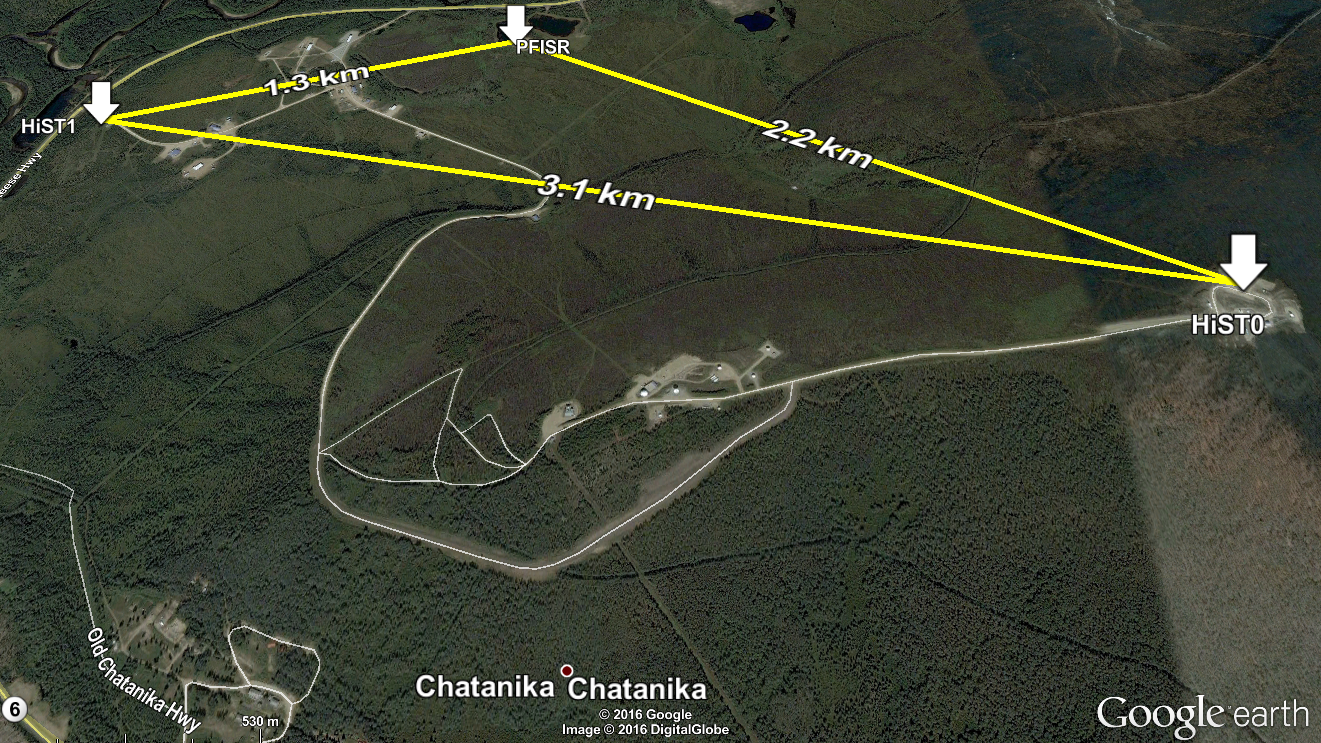
\includegraphics[width=\linewidth,trim=0 360 0 0,clip]{gfx/3sites}
	\caption{Location of HiST and PFISR at PFRR, Chatanika, AK. PFRR (65.1$^\circ$N, -147.5$^\circ$W) is \unit[30]{km} N-NE of Fairbanks, AK.}\label{fig:histloc}
\end{figure}
At PFRR, the inclination of the E-layer magnetic field is $77.5^\circ$, so the $B_\parallel$ axis is tipped $12.5^\circ$ from the local geographic vertical axis toward magnetic south.
The $B_\perp$ axis is defined to be orthogonal to $B_\parallel$ and coplanar with the cameras.
In auroral literature the ``width'' of auroral features refers to extent in the $B_\perp$ direction, and we follow this convention.

Prior work in auroral tomography \citep{jones1991,semeter1999,frey1998} has focused almost exclusively on mesoscale features of $\unit[10^4]{m}$ width recorded with typical sampling periods of order 1..\unit[30]{s}, with sensor baselines of 50..\unit[150]{km}.
The peak auroral emission intensity typically lies in the altitude range of approximately 100..\unit[300]{km}.
The $B_\parallel$ profile of the arc is dependent on the electron beam differential number flux and the characteristics of the neutrals and ions with which the precipitating particles interact.
An active auroral display embodies a vast hierarchy of spatial scales.
The global auroral oval is of order $\unit[10^5]{m}$ width as measured along magnetic latitude from the poleward to equatorward edges.
Dynamic fine-scale features embedded in an auroral breakup of $\unit[10^2]{m}$ width are typically observed during the substorm expansion phase \citep{semeter2008}.
Anthropogenic aurora of $\unit[10^2]{m}$ width has been observed from HAARP stimulus \citep{pederson2010,kendall2010}.
A complete theory of the aurora must account for variations at all scales inherent in the phenomena.
Although our theoretical understanding of global and mesoscale variability, and its drivers in the solar wind and magnetosphere, is well developed \citep{borovsky1993}, the physics underlying decameter-scale structure embedded within active auroral displays remains incomplete.

Auroral structures of sub-\unit[100]{m} width have been known to exist for decades \citep{maggsdavis1968,trondsendis}, and are seen regularly in long-term observations with modern cameras.
An example of a thin \unit[100]{m} wide auroral structure exhibiting rapid lateral motion is shown in the image sequence of Figure~\ref{fig:perspTrans}.
Note the substantial change in appearance of the arc in $1.5$ seconds, corresponding to a $5^\circ$ change in observer perspective, or about \unit[10]{km} in the $B_\perp$ dimension assuming \unit[120]{km} apparent auroral feature altitude.
%
An example of flaming aurora \citep{omholtbook,dahlgren2013} evolving over \unit[600]{ms} is shown in Figure~\ref{fig:perspFlame}.
%Both of these examples were recorded during the expansion phase of an auroral substorm.
%
% X1387_032307_112015.36_full_30fps.avi
% convert -normalize X1387*.avi[1132] 1132.png
% convert -normalize X1387*.avi[1147] 1147.png
% convert -normalize X1387*.avi[1162] 1162.png
% convert -normalize X1387*.avi[1177] 1177.png
% montage anno_11*.png -trim -tile 4x1 -geometry +1+0  anno_trans.png
\begin{figure*}\centering
    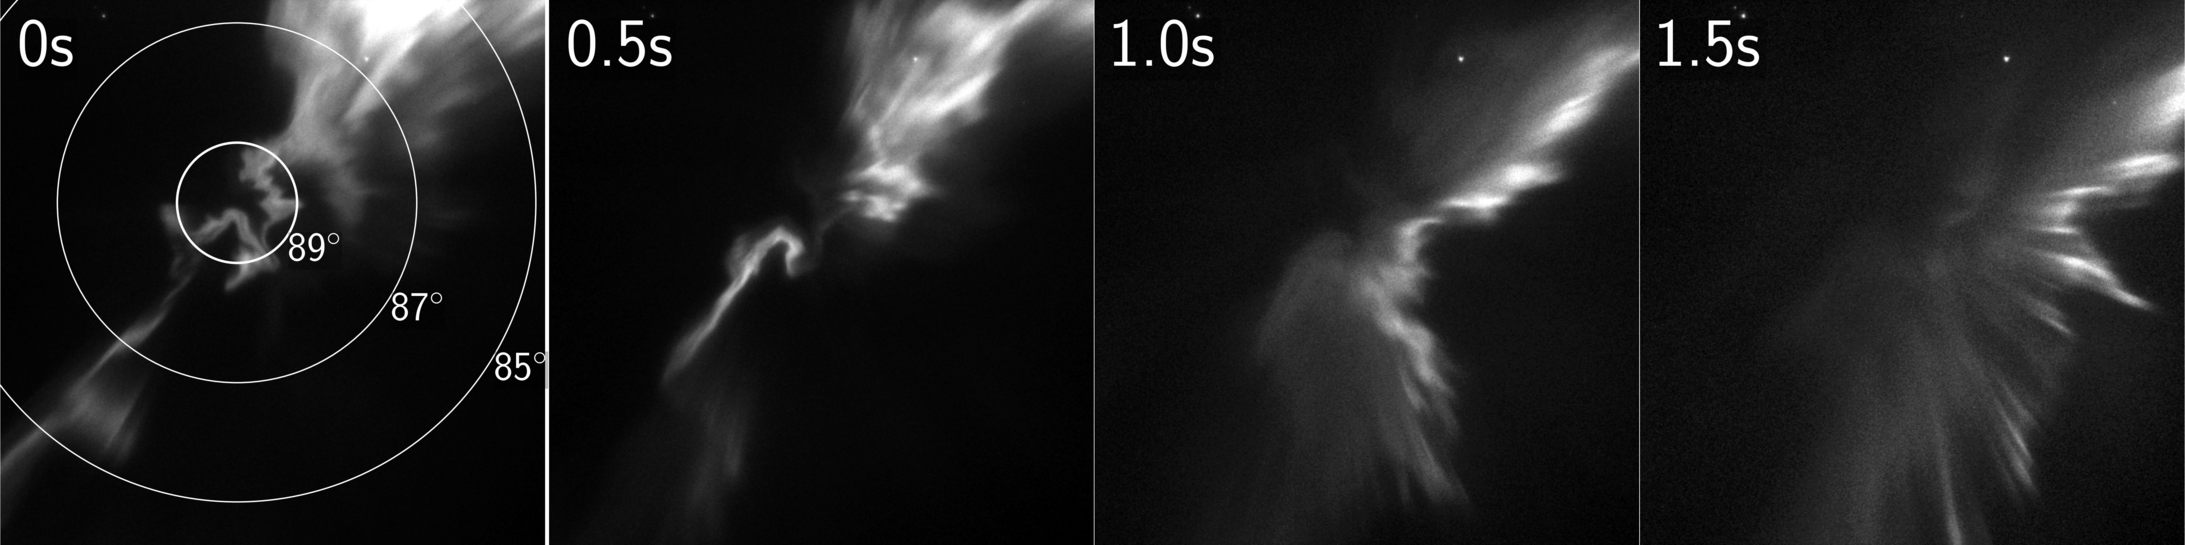
\includegraphics[width=\textwidth]{gfx/2007-03-23breakup}
    \caption{Radical change in perspective for \unit[100]{m} structure in \unit[1.5]{s} due to apparent $B_\perp$ transverse motion \citep{semeter2012,semeter2008}. 
    Contours are centered on local magnetic zenith.}
	\label{fig:perspTrans}
\end{figure*}
%
% generate figure 2.
%
% convert /tmp/CMOSvideo-0223.png -crop 900x550+880+610 flame100615440.png
% convert /tmp/CMOSvideo-0233.png -crop 900x550+880+610 flame100615640.png
% convert /tmp/CMOSvideo-0243.png -crop 900x550+880+610 flame100615840.png
% convert /tmp/CMOSvideo-0253.png -crop 900x550+880+610 flame100616040.png
% python fiducial.py
% montage anno_flame10061*.png -trim -tile 4x1 -geometry +1+0  anno_flame.png
%
%
\begin{figure*}\centering
    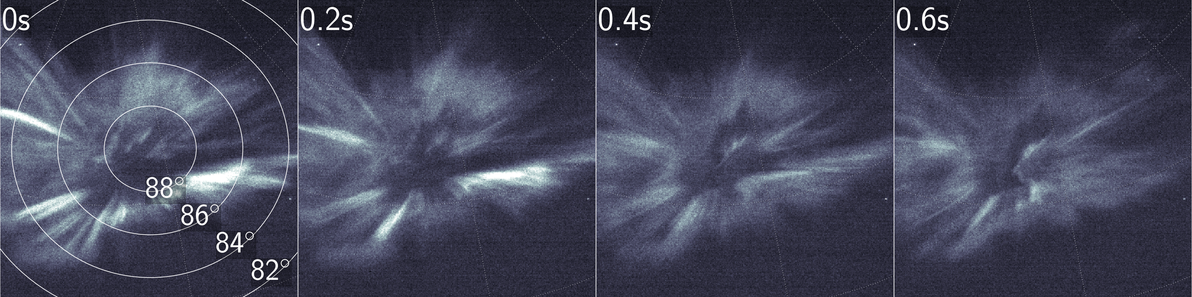
\includegraphics[width=\textwidth]{gfx/2011-03-01flame}
    \caption{Flaming aurora evolution over \unit[600]{ms} \citep{dahlgren2013}.
             Contours are centered on local magnetic zenith.}
    \label{fig:perspFlame}
\end{figure*}

Auroral acceleration occurs mainly in the altitude regime from 1000..\unit[40000]{km} \citep{lysak2011}, with DAW acceleration occurring mainly in the 1500..\unit[7000]{km} altitude range \citep{semeter2012}.
While the techniques of this system do not directly measure the acceleration regime, they do measure the outcomes of the acceleration.
The physics model based iterative reconstruction employed allows reconstructing particle flux at \unit[1000]{km} altitude, below which particle acceleration is negligible.
The reconstruction occurs over a sufficiently wide swath of sky (and can be widened by adding more cameras) to help characterize DAW structure in the lower magnetosphere.
%TODO block diagram showing magnetosphere

The tomographic techniques described in this dissertation contribute to understanding how such ephemeral fine-scale structure emerges in the incoming particle flux.
The observational requirements for a tomographic imaging system capable of resolving these scales are extreme, and the resulting inverse problem is highly ill-conditioned.
Section~\ref{sec:hist} presents the High Speed Tomography system (HiST) hardware \citep{hirsch2016}.
Sections~\ref{sec:flame} and~\ref{sec:transverse} comprise a feasibility study for a high frame-rate, short baseline, auroral tomography system.
Through simulation and modeling, we demonstrate that Electron Multiplying CCD (EMCCD) camera technology coupled with a physics-based regularization scheme is capable of resolving electron differential number flux dynamics of order \unit[100]{m} and \unit[10]{ms}.
The highest sensitivity cameras especially suitable for weak filtered auroral emissions are EMCCD-based.
EMCCD cameras are the core of the HiST system, along with GPSDO synchronization and embedded vision algorithms.

\section{Forward Model}\label{sec:fwd}
For the ill-conditioned problem produced by cameras with \unit[3]{km} spacing over \unit[100]{km} from the target of interest, regularization of the poorly observed vertical dimension is a necessary step to get a tractable inversion in terms of computational effort and error bounds.
We fashion a set of eigenprofiles from a problem comprised of linear differential equations by first making the assumption that production $p_{ij}$ and loss $l_{ij}$ for prompt emissions at steady state are related by
\begin{equation}\label{eq:continuity}
p_{ij} - l_{ij} = 0
\end{equation}
for the j\textsuperscript{th} excitation process of the i\textsuperscript{th} species.
The eigenprofiles are used as basis functions \citep{dahlgren2013} in a linear system tying together ground-observed auroral intensity to auroral volume emission rate via a known viewing geometry.
We can solve for the coefficients that correspond to the differential number flux for each log-spaced energy bin, yielding estimated differential number flux $\hat{\Phi}_{top}(B_\perp,E)$ for each new set of camera images.

To model the excitation rates due to primary electron precipitation, we use the 1-D TRANSCAR model \citep{lilensten2002,zett2007,zett2008,dahlgren2013,lummmerzheim1994}. 
Primary considerations for use of TRANSCAR include that 192 spectra are derived \citep{zettdis} from the excitation rates modeled by TRANSCAR. 
The use of a large number of spectra is important to maximizing the information available from a broadband optical filter such as the BG3 that passes numerous prompt line emissions.
The TRANSCAR hybrid kinetic/fluid time-dependent ionosphere model becomes more relevant in future studies incorporating joint observations with instruments such as incoherent scatter radar. 
Because a key requirement of the system is capturing order \unit[10]{ms} auroral dynamics, it was desirable to capture and incorporate the largest number of spectra possible to increase SNR at high frame rates.
TRANSCAR is a physics-based model of six positive ion species and their neutral parents: O\textsuperscript+, H\textsuperscript+, N\textsuperscript+, N$^+_2$, NO\textsuperscript+, O$^+_2$ along with electrons e$^-$ using the charge neutrality \citep{zett2007,blelly1996a,lilensten2002} of plasma $n_e = \sum_S n_s$. 
An 8-moment model \citep{blelly1996a} encompasses thermal diffusion effects so that important heat flows are captured \citep{zett2007}.
The TRANSCAR excitation rates and eigenprofiles used in this feasibility study are computed once for a particular set of geophysical parameters in an offline manner, which takes about 30 minutes using the idle CPU cycles of office PCs arranged in a compute cluster via GNU Parallel \citep{tange2011a}.
The rest of the forward model is implemented in about 2 seconds. 
The data inversion that must be executed for each observation time step must be done on-line for each new observation and takes about one minute on a desktop PC, depending on the number of cells in the projection matrix $\mathbf{L}$.

The close-spaced optical instruments used in this study yield persistent observations of precipitation process outcomes \citep{tanaka2011,wedlund2013} complementing on-orbit and rocket-borne \textit{in situ} measurements with a broader spatiotemporal context, along with improved $B_\perp$ resolution over widely spaced ground-based imagers.
Observation of a typical rapidly moving (several km/s) auroral feature implicitly requires a frame rate on the order of \unit[100]{Hz} for a narrow $9^\circ$ FOV and megapixel-class imager. 
Cameras comprising a multi-camera tomography system must have their frame start/end exposure times known to better than 1/10\textsuperscript{th} of a single frame.
Data inversion with poor time synchronization has limited scientific utility since the emissions observed at time $t_0$ at HiST0 will be smeared together with the results at time $t_0+\epsilon$ at HiST1 due to timing error $\epsilon$.
The camera site spacing is chosen based on the forward model described in this section along with practical facility availability. 

The auroral target of interest is taken to operate within the following first-order constraints:
\begin{enumerate}
    \item Auroral behavior in the $B_\parallel$ dimension is strongly influenced by time-dynamic electron particle penetration \citep{lilensten2002}, as modeled by TRANSCAR. Time of flight difference between high energy and low energy particles in the lower magnetosphere at time scales less than order \unit[10]{ms} have been observed \citep{peticolas2000}. 
    The tomographic process gives information on vertical structure not available in zenith-oriented line integrations alone as in \citet{peticolas2000}, so our technique will capture dynamics with frame rates to at least \unit[100]{Hz}.
    \item Precipitating e\textsuperscript{-} acceleration has taken place above the uppermost altitude cell of the 1-D model, implying that thermospheric and mirroring forces are neglected \citep{lilensten2002,swift1975}
    \item Auroral behavior in the $B_\perp$ dimension is dominated by collisionless processes above the ``top'' of the ionosphere (altitude $>1000$~km) \citep{mozer1998,ergun2002}
\end{enumerate}
With these constraints in mind, we continue with a discussion of the quantitative particulars of the models and algorithms used in this feasibility study. 

%
\begin{figure}\centering 
    %the \par is necessary after each text to make the \baselineskip take effect
    \begin{tikzpicture}[node distance=2cm, auto]
    
    \node (in) [startstop, text width=4.5cm] {\baselineskip=10pt e\textsuperscript{-} Precipitation $\Phi_{top}$ \par};
    \node (p) [process, below of=in, text width = 4.5cm,yshift=-0.5cm] {\baselineskip=12pt Excitation $\Rightarrow$ Prompt Emissions \[ p_\lambda(z) \propto p_{ij}(z) \] \par };
    \node (B) [process, below of=p, text width=6cm, yshift=-1.25cm]{\baselineskip=10pt Image Intensity \begin{align*} 
    	\mathscr{I} =&   \int_0^\infty \int_\lambda p(\lambda,\mathbf{\ell}) M(\lambda) \mathrm{d} \lambda \mathrm{d}\ell \\
    	\mathbf{I} =& \tau a g \mathscr{I}
    	\end{align*}
    	\par};
    %
    \node (eig) [compute, right of=in, text width=3.cm,xshift=5.cm] {\baselineskip=10pt Eigenprofiles $\mathbf{T}(E,z)$ \par};
    \node (P) [compute, below of=eig, text width=4cm,yshift=0.4cm] {Volume Emissions $\mathbf{P} = \mathbf{T}\Phi$};
    \node (L) [compute, below of=P, text width=4cm,yshift=0.4cm] {Projection Matrix $\mathbf{L}$};
    \node (min) [estimate,text width=5.5cm, below of=L,yshift=-0.5cm] {\baselineskip=12pt Estimate  \begin{align*} \hat{\Phi}_{top} &= \argmin_\Phi ||\mathbf{I}-\mathbf{LT}\hat{\Phi}_{top}||_2 \\
        \hat{E}_0 &= \argmax_E \hat{\Phi}_{top} \\
        \hat{B}_{\perp,0} &= \argmax_{B_\perp}  \hat{\Phi}_{top}
        \end{align*} \par};
    
    %
    \draw[arrow] (in) -- (p);
    \draw[arrow] (p) -- (B);
    \draw[arrow] (B) -- (min);
    %
    \draw[arrow] (eig) -- (P);
    \draw[arrow] (P) --(L);
    \draw[arrow] (L) -- (min);
    \end{tikzpicture}
    \caption{Block diagram of HiST auroral tomography forward model and data inversion.}
    \label{fig:overall}
\end{figure}

Referring to the left column of Figure~\ref{fig:overall}, the forward model input $\Phi_{top}$ is generated using a parameterization \citep{strickland1993} with representative values shown in Figure~\ref{fig:fwdstrick}, where the location in energy of peak differential number flux is known as the characteristic energy $E_0$.
%
% python gridaurora/eFluxGen.py ../histfeas/in/demo_flux.h5
\begin{figure}\centering
    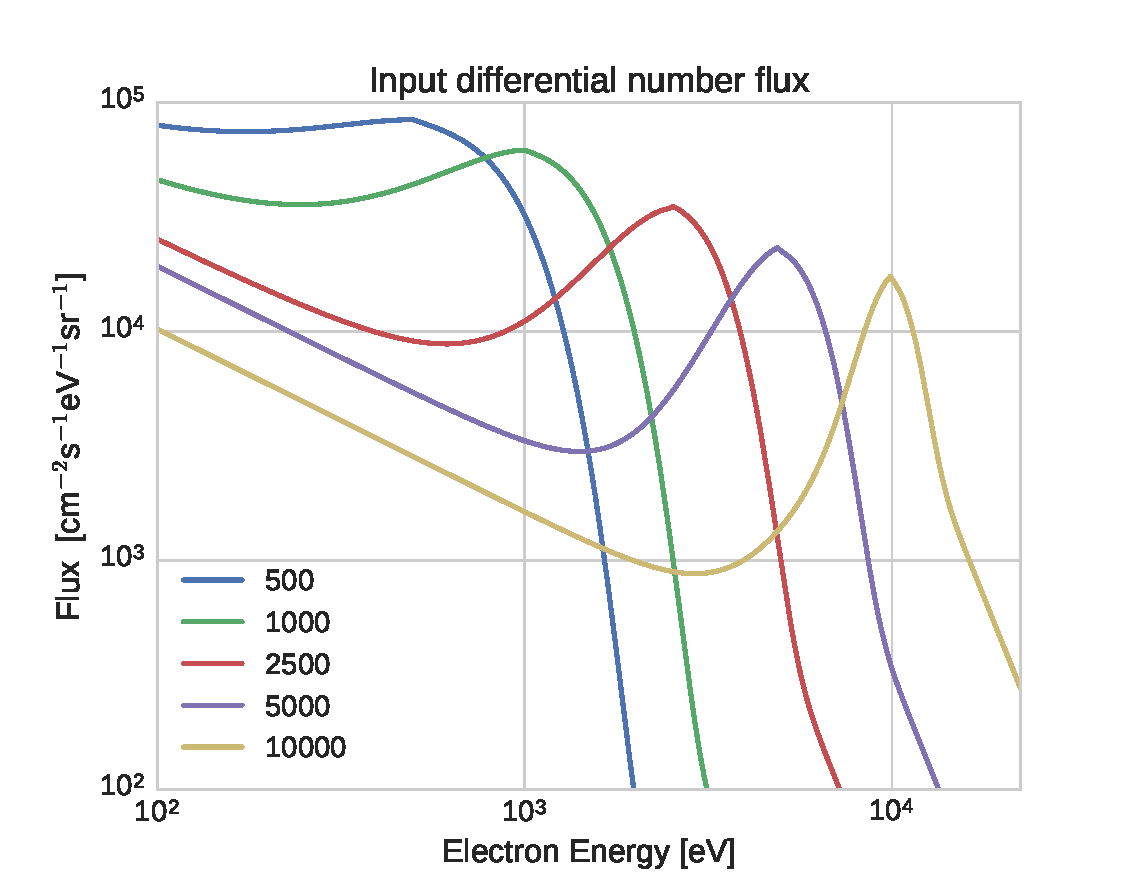
\includegraphics[width=\columnwidth,trim=0 0 50 20,clip]{gfx/hirsc6}
    \caption{Input differential number flux for beams with $E_0\in$ \{500, 1000, 2500, 5000, 10000\}~eV \citep{strickland1993}.}\label{fig:fwdstrick}
\end{figure}
%
The physical process generating $p_\lambda(z)$ in the second block of the left column of Figure~\ref{fig:overall} is modeled in TRANSCAR \citep{zett2007,blelly1996a,lilensten2002} and represented by the eigenprofiles $\mathbf{T}$ in the upper right block of Figure~\ref{fig:overall}, with line-integrated modeled spectra for each beam energy shown with and without BG3 filtering in Figure~\ref{fig:spectra}.
%
% python test_calcemissions.py ~/code/histfeas/test/data/ 1613.5 -t 0 -m spectra1d
%
\begin{figure}
    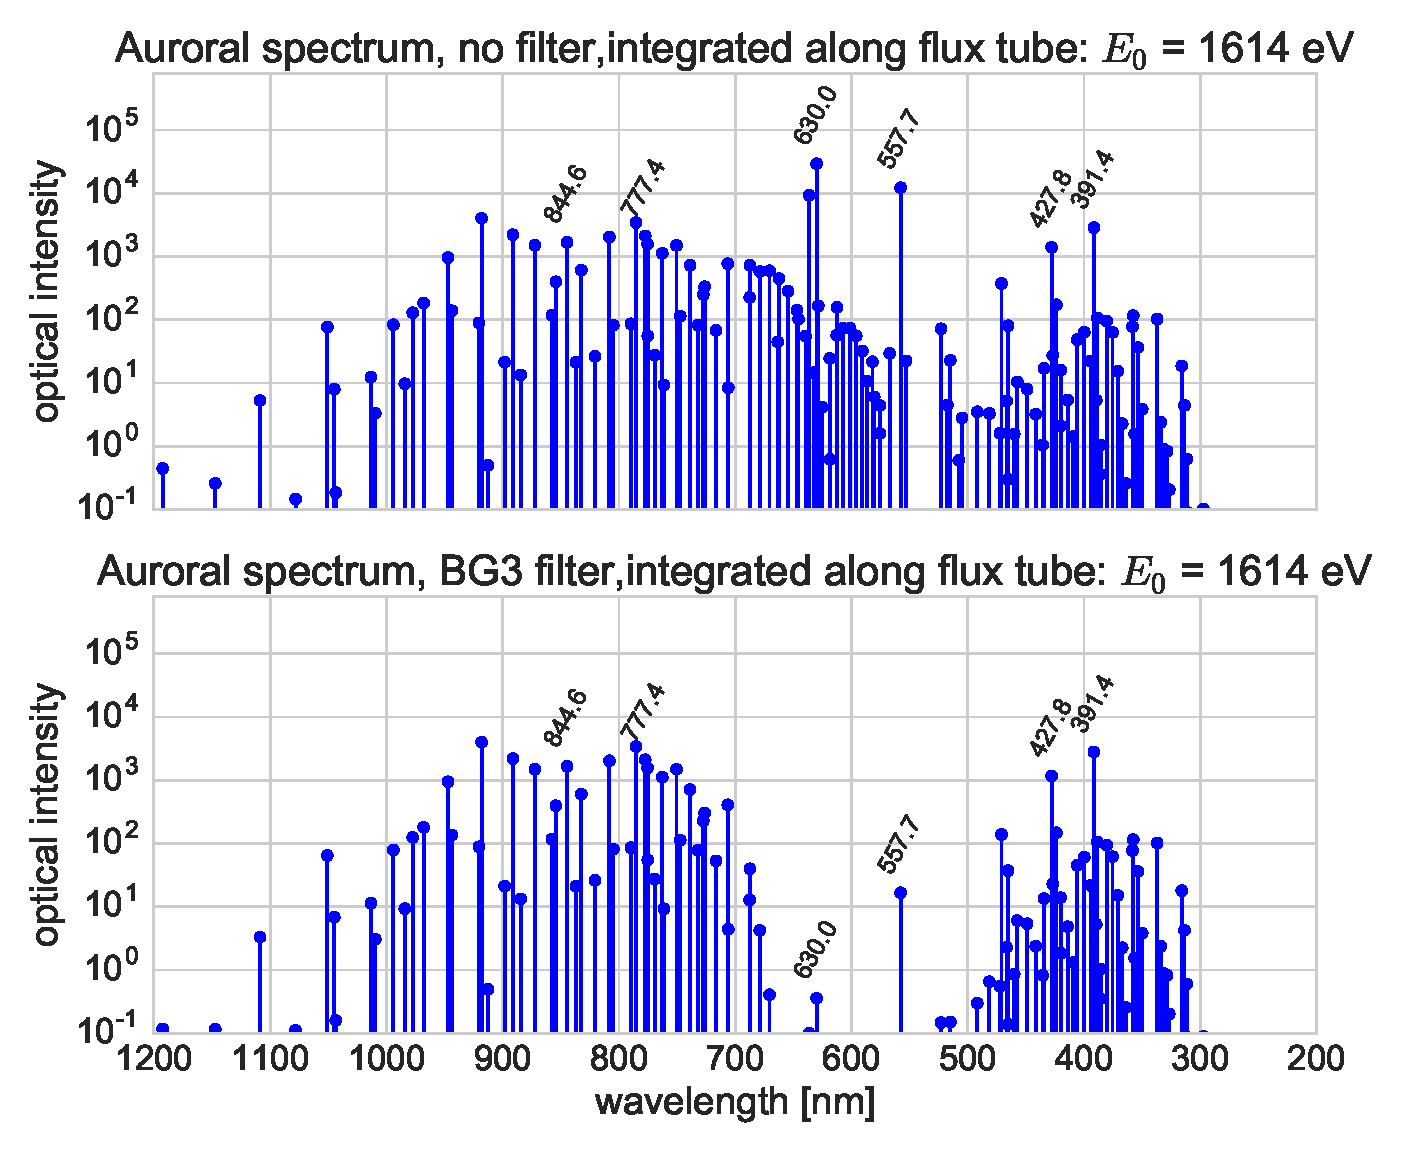
\includegraphics[width=\columnwidth,trim=0 10 0 0,clip]{gfx/hirsc7}
    \caption{Auroral Spectrum integrated along flux tube for $E_0=1.6$~keV, with and without BG3 filter.}\label{fig:spectra}
\end{figure} 
%
Some of the brightest features in the aurora are produced by metastable transitions with radiative lifetimes of order \unit[1..10]{s} \citep{vallancejones1974}. 
In Alfvénic aurora, the electron flux rapidly changes ($< \unit[10]{ms}$ scales) in $B_\perp$ and $E_0$, and the intense metastable emissions glow like an high-persistence oscilloscope phosphor, which in a white light sensor can cover up the much fainter prompt emissions that have several orders of magnitude shorter lifetimes.
Each camera was equipped with a BG3 optical filter with the transmission characteristics of Figure~\ref{fig:optTrans} to greatly attenuate these long lifetime features.
In particular, the deep notch in transmission for the long lifetime metastable emissions lines includes \unit[557.7]{nm} and \unit[630]{nm}.
%
% python gridaurora/test_opticalmod.py -m eps
\begin{figure}\centering
    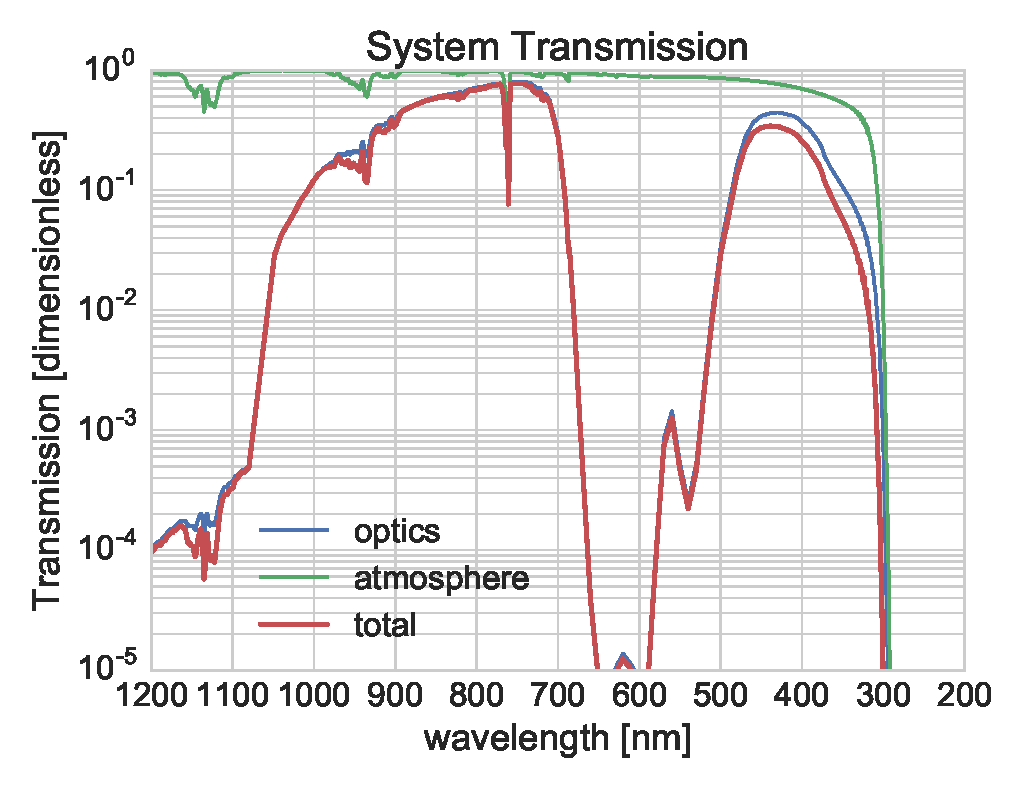
\includegraphics[width=\columnwidth,trim=5 5 5 5,clip]{gfx/hirsc8}
    \caption{Optical system transmission, including BG3 filter, EMCCD window and LOWTRAN modeled atmospheric absorption.}\label{fig:optTrans}
\end{figure}
%
The volume production rate of process $p_{ij}$ integrated over fixed pitch angle $\mu$ resulting from the TRANSCAR model is 
\begin{equation}\label{eq:prodEq2}
p_{ij}(z) =n_i(z) \int \sigma_{ij}(E)\Phi(z,E)\textrm{d}E 
\end{equation}
where $n_i$ is the MSIS90-initialized density of the i\textsuperscript{th} ground-state neutral species (e.g. N$_2$, O$_2$, O). $\sigma_{ij}$ is the electron impact cross section of the $j$\textsuperscript{th} excitation process for the $i$\textsuperscript{th} species \citep{semeter2012}. 
$\Phi(z,E)$ is the pitch angle integrated flux obtained from the 1-D model TRANSCAR \citep{blelly1996a} for 33 log-spaced energy bins $E$ ranging from \unit[58]{eV} to \unit[17.7]{keV} \citep{dahlgren2013}. 
For prompt emissions, we connect excitation rates to optical volume emission rates using~\eqref{eq:continuity} with \citep{zettdis,vallancejones1974} the Einstein coefficients and Franck-Condon factors,
\begin{equation}\label{eq:prompt4}
p_\lambda(z) \propto p_{ij}(z)
\end{equation}

For the lower left block of Figure~\ref{fig:overall}, the photon flux at the $k$\textsuperscript{th} camera pixel is described by a line integral mapped via the lens to angle $\theta_k$, treating the auroral region as optically thin at the wavelengths observable through the optical filtering and LOWTRAN \citep{lowtran7} modeled atmospheric absorption of Figure~\ref{fig:optTrans}.
Considering~\eqref{eq:prompt4} and total transmission $M(\lambda)$ shown in Figure~\ref{fig:optTrans}, the photon flux available at the imaging chip $\mathscr{I}(\theta)$ is
\begin{equation}\label{eq:grayb}
\mathscr{I}(\theta) =  \int_0^\infty \int_\lambda p(\lambda,\mathbf{\ell}) M(\lambda) \textrm{d} \lambda \textrm{d}\ell
\end{equation}
The camera exposure time $\tau$, amplifier gain $g$ and pixel area $a$ are modeled with the output in data numbers $\mathbf{I}$ as:
\begin{equation}\label{eq:dn}
\mathbf{I} = \tau a g \mathscr{I}
\end{equation}
where typical values include $a=(16~\mu\textrm{ m})^2, \tau = 2\times10^{-2}~\textrm{s}, g=1~I / \textrm{e}^- $.

Referring to the right column of Figure~\ref{fig:overall} we assemble projection matrix $\mathbf{L}$ by mapping viewing angle $\theta$ to our discrete EMCCD imaging arrays, and compute the intersection length of each ray \citep{semdis} with the relevant cell of $\mathbf{L}$ using the Cohen-Sutherland line clipping algorithm \citep{cohensutherland,cvutils}.
The dimensions of $\mathbf{L}$ are $N_{cam} N_{cut} \times N_{B_\perp} N_{B_\parallel}$,  where $N_{cam}$ is the number of cameras in the system, $N_{cut}$ is the number of 1-D pixels used from each camera and $N_{B_\perp},N_{B_\parallel}$ are the number of $B_\perp, B_\parallel$ pixels in the grid for the volume emission rate matrix $\mathbf{P}$ .
The IGRF 11 model is incorporated into $\mathbf{L}$ for the Poker Flat Research Range, where the inclination $77.5^\circ$ and declination $19.9^\circ$ of the local geomagnetic field determine the angular coördinates of magnetic zenith. 

The grid of Figure~\ref{fig:Lcam} extends from approximately 90-1000~km altitude, showing the locations used in estimating volume emission rate $\mathbf{P}$ due to the incident differential number flux $\Phi_{top}$.
\begin{figure}
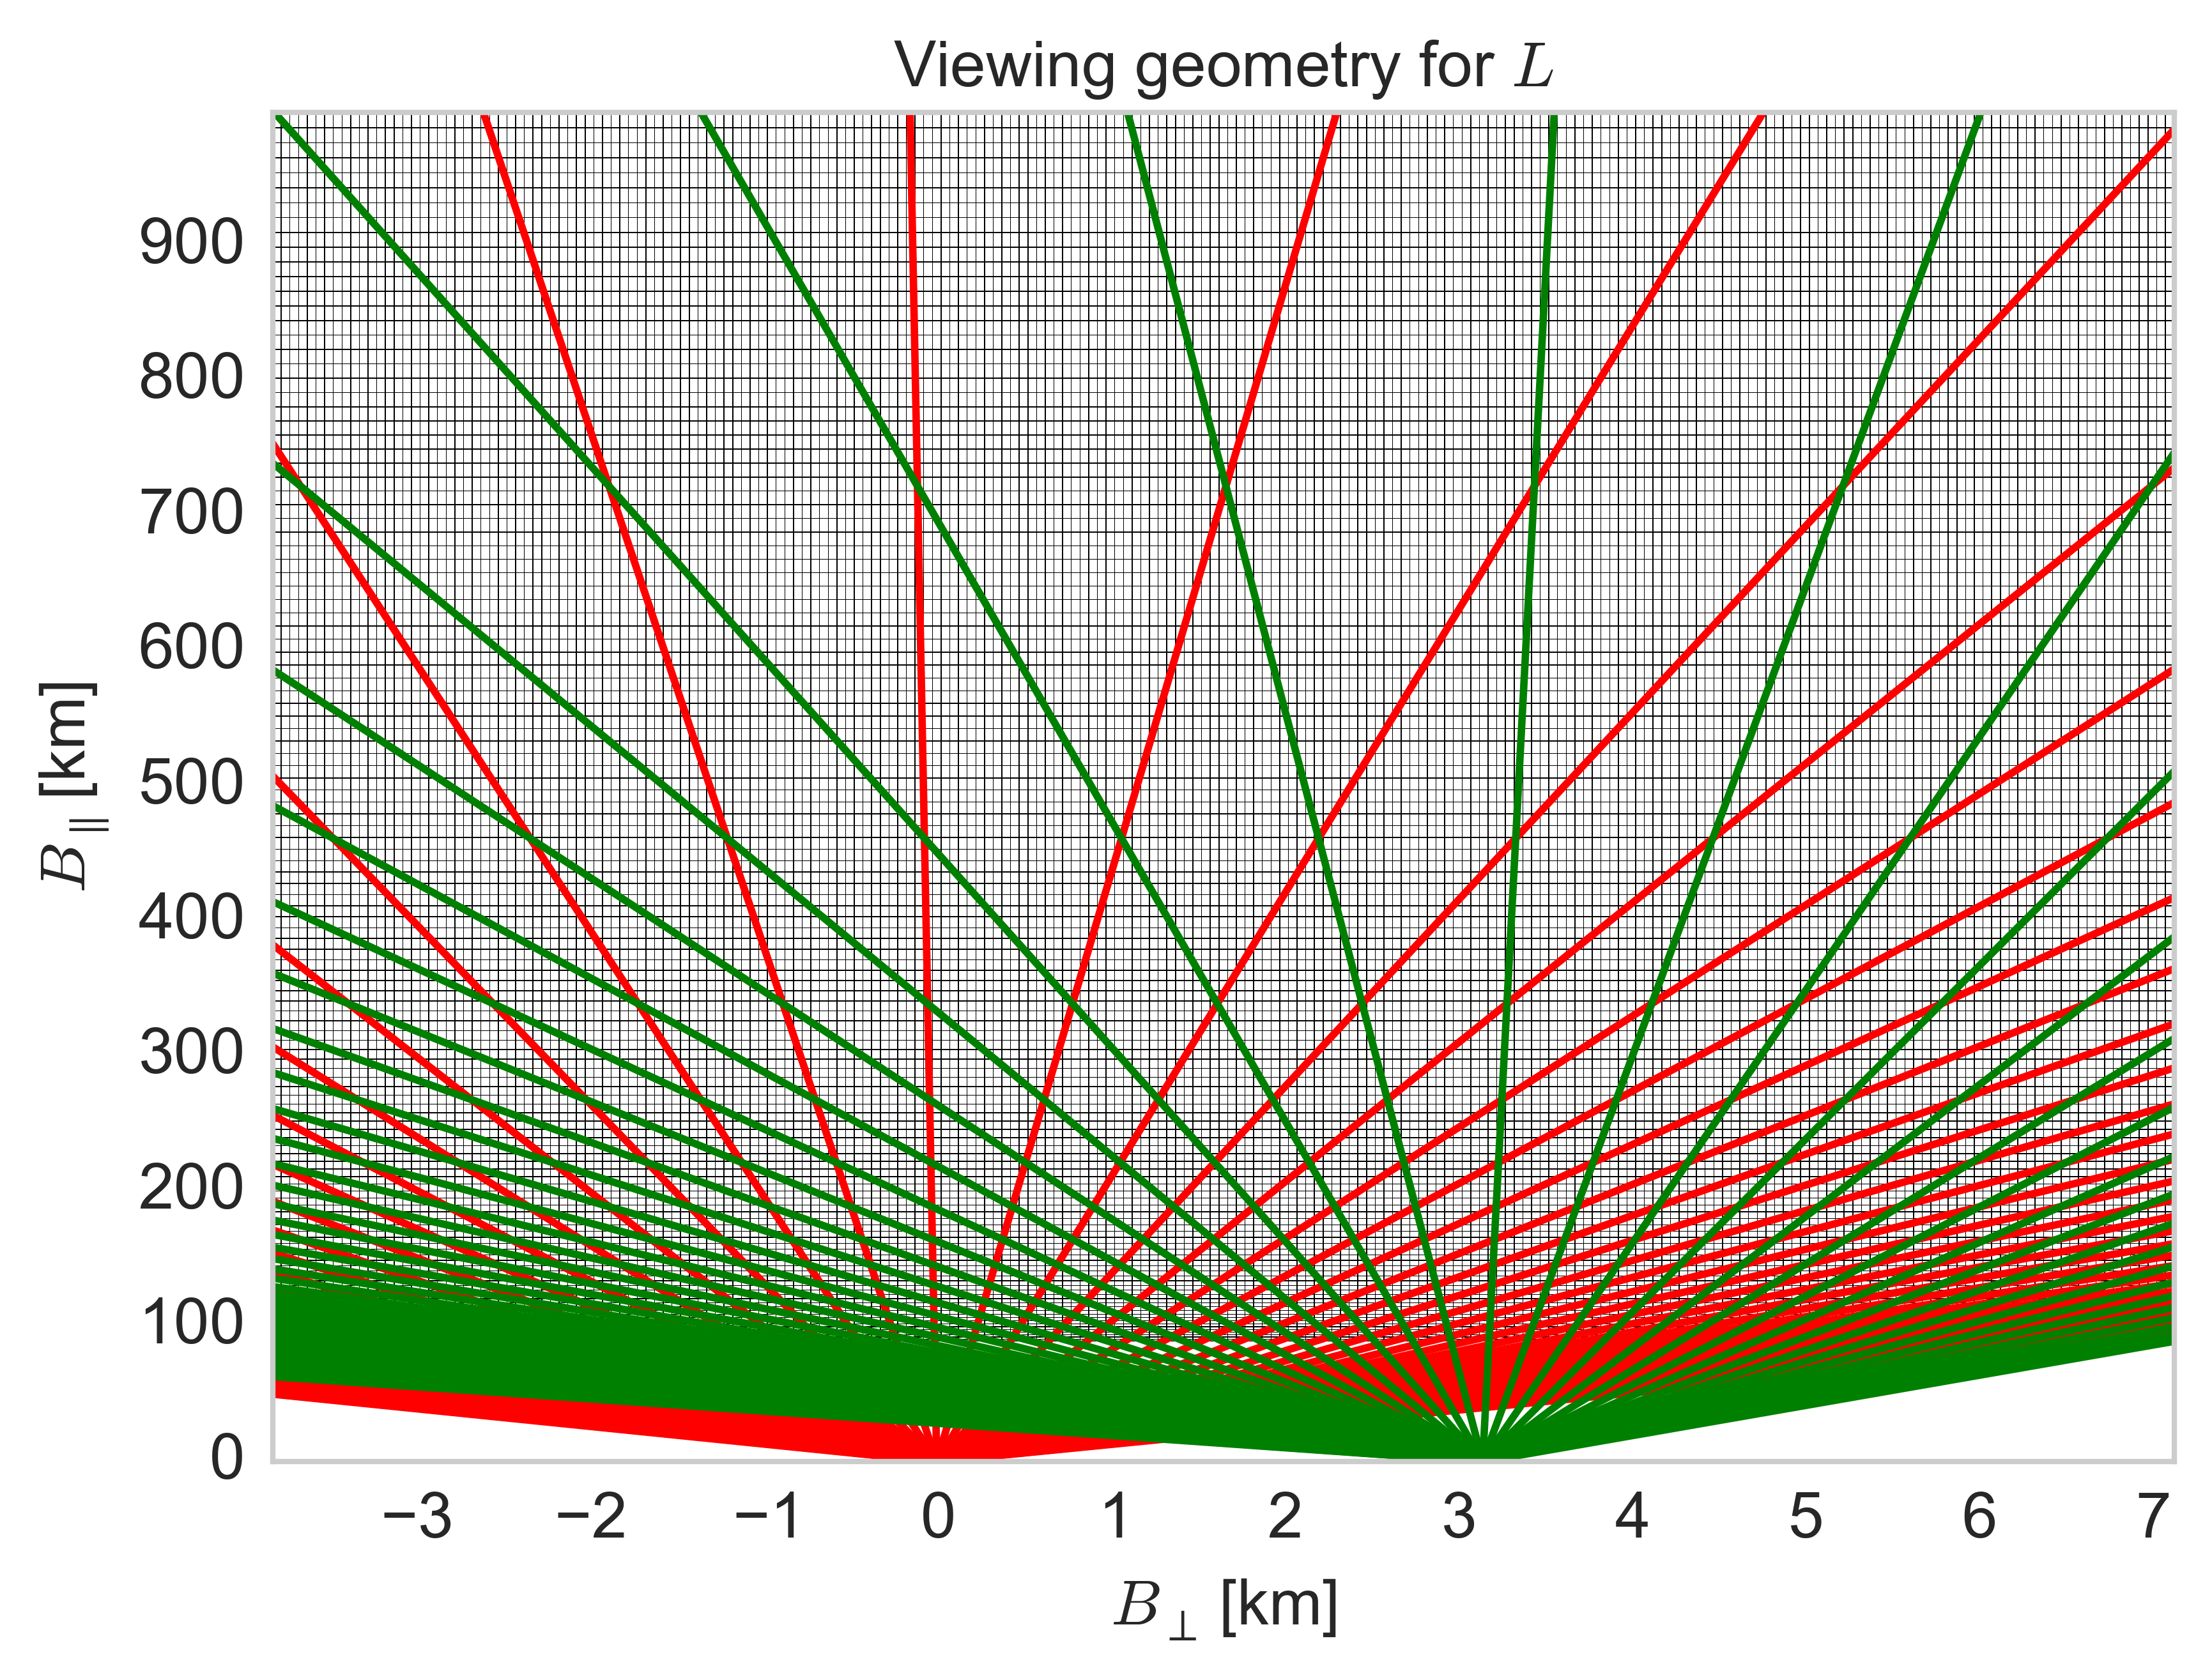
\includegraphics[width=\columnwidth,trim=5 6 5 5,clip]{gfx/Lcam}
\caption{Viewing geometry for the two-camera system at the Poker Flat Research Range, showing selected lines of sight over a decimated reconstruction grid.}\label{fig:Lcam}
\end{figure}
Overlaid on this grid are the decimated 1-D rays corresponding to intensity vector $\mathbf{I(\theta)}$.
For Figure~\ref{fig:Lcam} and the analysis of Section~\ref{sec:transverse} and~\ref{sec:flame}, $N_{cam}=2, N_{cut}=512, N_{B_\perp}=219, N_{B_\parallel}=123$.
This forward model yields ground-observed optical intensity vs. angle due to electron differential number flux $\Phi_{top}(B_\perp,E)$. 
The analysis in Section~\ref{sec:inv} uses observations from ground-based cameras to estimate the unobservable differential number flux $\hat{\Phi}_{top}$ via a minimization algorithm. 

\section{HiST Data Inversion}\label{sec:inv}

To estimate the characteristics of the time-dependent differential electron number flux $\Phi_{top}$ high in the ionosphere where collisionless processes dominate we employ a physics-based regularization scheme. 
The poorly observed $B_\parallel$ dimension is regularized with a linear basis expansion of volume emission rate eigenprofiles calculated by the TRANSCAR model.
The 33 log-spaced energy bins from \unit[58]{eV} to \unit[17.7]{keV} each have a coefficient estimated by our inversion algorithm for each $B_\perp$ location, comprising $\hat{\Phi}_{top}(B_\perp,E)$.
For the simulations of chapter~\ref{chapter:sim}, $\hat{\Phi}_{top}$ has dimensions $(219,33)$.
Regularization along $B_\parallel$ is key to finding a physically plausible solution from the infinitely many possible solutions due to the large null space of the inverse problem.
The data inversion process is outlined in the right column of Fig.~\ref{fig:overall}.
As observed in the middle row of Fig.~\ref{fig:est1dflame}, the volume emission rate is a smooth function of differential number flux and altitude.
The smoothness justifies describing the relationship between the unobservable \textit{in situ} physics and the observable auroral intensity by the Fredholm Integral of the First Kind,
%
\begin{equation}\label{eq:fiefk}
g(s) = \int_a^b K(s,t)f(t)\textrm{d}t
\end{equation}
%
where $f(t)$ is the unknown quantity, $g(s)$ is the observed quantity, and $K(s,t)$ is the kernel through which $g(s)$ is observed, encompassing optical filters, line integration of volume emission rate, and noise. 
For the present auroral tomography problem, we incorporate TRANSCAR eigenprofiles
\begin{equation}\label{eq:eigentranscar}
T(E,z) = \int_{\lambda} p_\lambda(E,z) M(\lambda) \textrm{d}\lambda
\end{equation}
in a representation of total auroral volume emission rate as
%
\begin{equation}\label{eq:fiefkE}
P(z) = \int_0^\infty T(E,z) \Phi_{top}(E)\textrm{d}E
\end{equation}
%
which has the same form as~\eqref{eq:fiefk} and may be discretized in matrix form,
%
\begin{equation}\label{eq:fiefkEmat}
\mathbf{P} = \mathbf{T}\Phi_{top}
\end{equation}
%
The discretized forms are convenient for computer implementation since the continuous integration~\eqref{eq:fiefkE} is represented by matrix multiplication~\eqref{eq:fiefkEmat}.
The BG3 filtered and atmosphere attenuated continuüm of wavelengths is observed at the camera as grayscale intensity
%
\begin{equation}\label{eq:master}
\textbf{L}\textbf{T}\Phi_{top}=\textbf{I}
\end{equation}
resulting in the data numbers $\mathbf{I}$ of~\eqref{eq:dn}.

In general $\mathbf{L}$ and $\mathbf{T}$ are not square, so the inverse $\mathbf{L}^{-1}$ and $\mathbf{T}^{-1}$ are not defined in this underdetermined system.
The ill-conditioned and Hadamard ill-posed nature of the problem arises both from the extreme problem geometry and that there is not a unique tomographic solution for the incident number flux causing an auroral display.
A method for solving such problems via brute force is the use of minimization algorithms \citep{semeter1997}. 
The algorithm selected for this effort is the Limited Memory Broyden-Fletcher-Goldfarb-Shanno algorithm \citep{Byrd1995,Zhu1997,Morales2011}, known as L-BFGS-B \citep{scipy}.
This algorithm was selected based on fast convergence for the large number $(>7000)$ of $\hat{\Phi}_{top}(B_\perp,E)$  parameters to minimize based on an empirical comparison with other contemporary minimization techniques.

For a particular realization of geophysical conditions and choice of differential number flux energy bins $\mathbf{T}$ is obtained from an off-line computation. 
As implicit in \eqref{eq:fiefk}, $\mathbf{T}$ is identical in the forward model and data inversion.
The 1-D slices of the synchronized images from each camera are stacked in column-major vector $\mathbf{I}$. 
The 2-D array $\hat{\Phi}_{top}(B_\perp,E)$ has rows arranged by precipitation energy in eV and columns arranged by $B_\perp$ location in kilometers.
We use L-BFGS-B minimization function
\begin{equation}\label{eq:bmin}
\hat{\Phi}_{top}(B_\perp,E) = \argmin_\Phi||\mathbf{I}-\mathbf{LT}\hat{\Phi}_{top} ||_2 =  \argmin_\Phi ||\mathbf{I}-\hat{\mathbf{I}}||_2
\end{equation}
with the bounds $\Phi \in \left[0,\infty\right)$ is given an initial guess $\Phi_{top}(B_\perp,E) \equiv 0$, and is allowed to run for 10--20 cycles. 
Automated measurements of $E_0$ and $B_{\perp,0}$ are accomplished via a 2-D Gaussian fitter algorithm originally based on MINPACK \citep{Minpack}. 
The region of the maximum differential number flux is fitted with a 2-D Gaussian using a Levenberg-Marquardt least squares algorithm to find the parameters best fitting the peak vicinity of $\hat{\Phi}_{top}$. 
In general, the forward model will have limitations in absolute accuracy with regard to the physical world due to the model assumptions and simplifications necessary to get a tractable computation within time and memory constraints.
We now examine simulations of two types of highly dynamic auroral events to show the feasibility of the HiST system for estimating $E_0$ and $B_{\perp,0}$.

%\section{ISR Data Inversion}\label{sec:isrinv}
Recent work on inversion of auroral observations to estimate the incident precipitation energy flux distribution at the top of the ionosphere includes \citet{zett2007,semeter2012,dahlgren2013,wedlund2013,hirsch2016}. 
An overview of the inversion process needed is
\begin{equation}\label{eq:fiefk1}
\vec{q} = \mathbf{A}\vec{\phi}
\end{equation}
where $\vec{q}$ is a $z \times 1$ column vector of ionization rates--ionization caused by electron precipitation into the ionosphere, and
\begin{equation}\label{eq:fiefk2}
\vec{P} = \mathbf{B} \vec{\phi}
\end{equation}
where $\vec{P}$ is a $z \times 1$ column vector of VER caused by kinetic interactions of precipitating electrons with the ionosphere \citep{wedlund2013}.

The electron precipitation is represented by $\vect{\phi}$, an $E \times 1$ column vector of ionization rates. 
$z$ is the number of altitude bins chosen in the discrete problem. 
$E$ is the number of differential energy bins chosen in the discrete problem. 
$\mathbf{A}$ and $\mathbf{B}$ are each of dimensions $z \times E$.





\citet{partamies2004} omits secondary electrons, since they have energies of less than 100 eV. % [p. 1968 last paragraph]
A significant portion of energy observed by the \unit[32]{eV}..\unit[30]{keV} DMSP particle detector is above \unit[8]{keV} \citep{partamies2004}. % [p.1969 first para].
p. 1964 $$ 1\textrm{mW/m}^2 = 6.24\times10^{12} \textrm{keV/m}^2\textrm{s} $$

\citet{partamies2004} used SPECTRUM, a non-standard FORTRAN 77 program translated by Annika Olsson to Matlab to calculate energy fluxes from the $N_e$ measured by ISR.
\url{http://www.lunduniversity.lu.se/lucat/user/54539ff9da4c67bb5baee00c09f22816}
\url{ftp://ftp.irf.se/pub/perm/ESRAD/SPECTRUM/}



% python figure_flame2.py --load -m fwd optim eps 

\section{Model and Inversion of Flaming Aurora}\label{sec:flame}
We model two time steps of a flaming auroral event with $E_0\in\lbrace{4.5,1.6\rbrace}$~keV. 
The input differential number flux $\Phi_{top}$ is shown in Fig.~\ref{fig:estflame}(a)(c). 
Fig.~\ref{fig:estflame}(b)(d) show the estimated differential number flux $\hat{\Phi}_{top}$ using the L-BFGS-B algorithm. 
%
\begin{figure}\centering
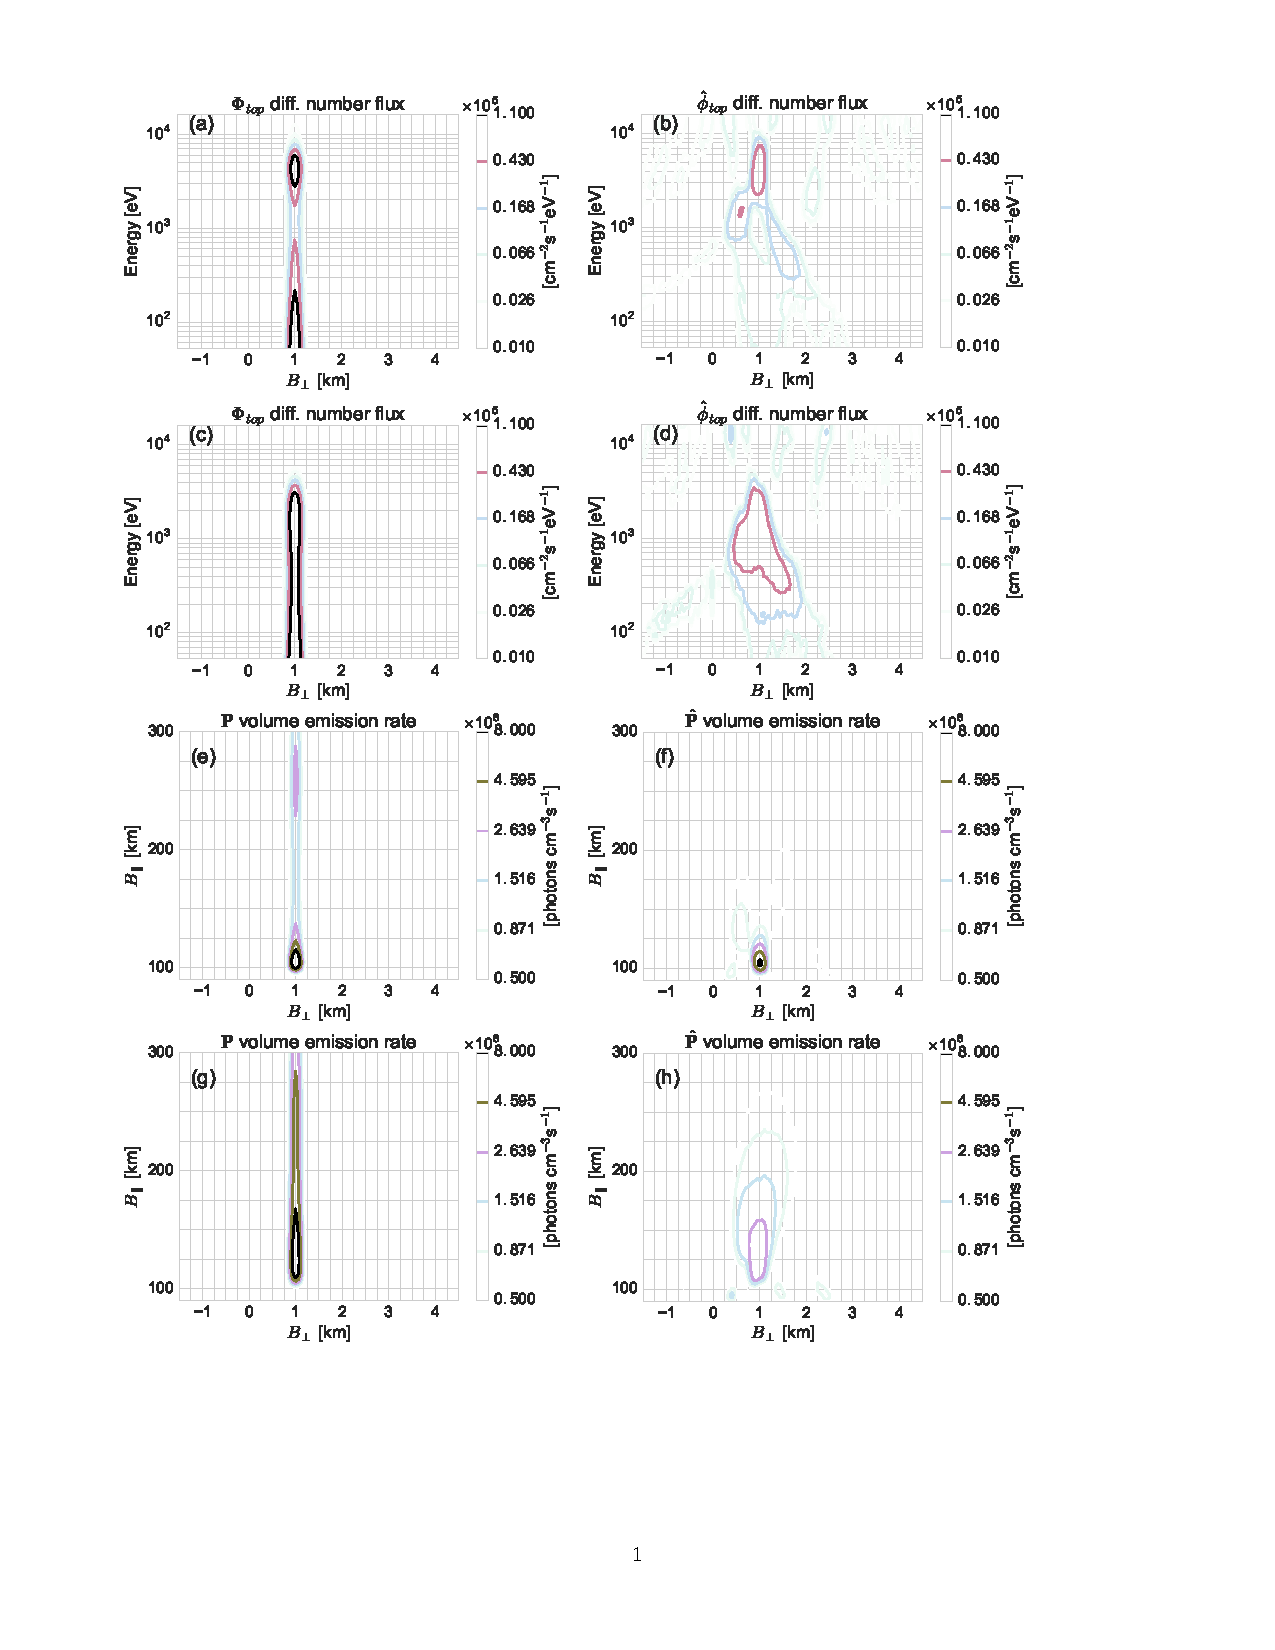
\includegraphics[trim=30 120 100 20,clip,height=0.85\textheight]{gfx/flamesim}
\caption{Flaming aurora simulation with characteristic energy $E_0\in\{4.5,1.6\}$~keV and $B_{\perp,0}=1.0$~km. 
(a)(c): differential number flux $\Phi_{top}$. (b)(d): estimated differential number flux $\hat{\Phi}_{top}$. 
(e)(g): forward modeled VER $\mathbf{P}$.  (f)(h): estimated VER $\mathbf{\hat{P}}$.} \label{fig:estflame}
\end{figure}
%
1-D cuts of $\Phi_{top}$ and $\hat{\Phi}_{top}$ at $B_{\perp}=1.0$~km are shown in Fig.~\ref{fig:est1dflame}(a)(b) respectively to aid in visualizing the characteristic energy $E_0$.
Table~\ref{tab:Jestflame} describes the $E_0$ estimation error.
%
\begin{sidewaystable}\centering
\caption{Simulated estimation error for flaming and translating auroral arcs.} \label{tab:Jestflame}
	\begin{tabular}{llllll}
		\toprule
		$B_{\perp,0}$ [km] & $E_0$ [keV] & $\hat{B}_{\perp,0}$ [km] & $\hat{E}_0$ [keV] & Error $|B_{\perp,0}-\hat{B}_\perp,0|$ [\%] & Error $|E_0-\hat{E}_0|$ [\%] \\
		\midrule
		1.0 & 4.5 & 1.0 & 4.1 & \textless 5 & \textless 10 \\
		1.0 & 1.6 & 1.0 & 1.7 & \textless 5 & \textless 10 \\
		1.55 & 5.0 & 1.55 & 4.67 & \textless 5 & \textless 10 \\
		2.5 & 4.5 & 2.5 & 4.1  & \textless 5 &  \textless 20  \\ 
		2.5 & 1.6 & 2.55 & 1.2 & \textless 5 &  \textless 25  \\ 
		3.75 & 5.0 & 3.7 & 5.7 & \textless 5 & \textless 25 \\
		4.2 & 4.5 & 4.15 & 5.6  & \textless 5 &  \textless 25  \\
		4.2 & 1.6 & 4.1 & 1.15  & \textless 5 &  \textless 30  \\
		\bottomrule
	\end{tabular}
	
\end{sidewaystable}

The estimated volume emission rate $\hat{\mathbf{P}}$ as shown in Figure~\ref{fig:estflame}(f)(h) and as 1-D cuts in Figure~\ref{fig:est1dflame}(c)(d) have morphologically similar characteristics to the forward modeled volume emission rate $\mathbf{P}$ in Figure~\ref{fig:est1dflame}(e)(g), as expected.
We observe that the estimated ground-observed intensity $\hat{\mathbf{I}}$ in Figure~\ref{fig:est1dflame}(e)(f) is within a small factor of the forward model intensity $\mathbf{I}$. 
As summarized in Table~\ref{tab:Jestflame}, $\hat{\Phi}_{top,0}$ has been estimated with $E_0$ error typically less than 30\% for simulated auroral arcs within $2.5^\circ$ of magnetic zenith.

The addition of a third camera at $B_\perp=\unit[10]{km}$ initially does not appear to make a dramatic improvement in increasing the angular range from magnetic zenith for estimating $\hat{\Phi}_{top,0}$. 
It is desirable to extend the estimate of precipitation characteristics to 3-D, which intrinsically motivates incorporating more than 2 cameras into HiST.
As observed in Table~\ref{tab:Jestflame}, the $\hat{\Phi}_{top,0}$ estimate is usable to at least $2.5^\circ$ from magnetic zenith.
It is apparent that a key limit of the $B_\perp$ range of the inversion is keeping the auroral target within the common FOV of the cameras, as is trivially expected. 


\begin{figure}\centering
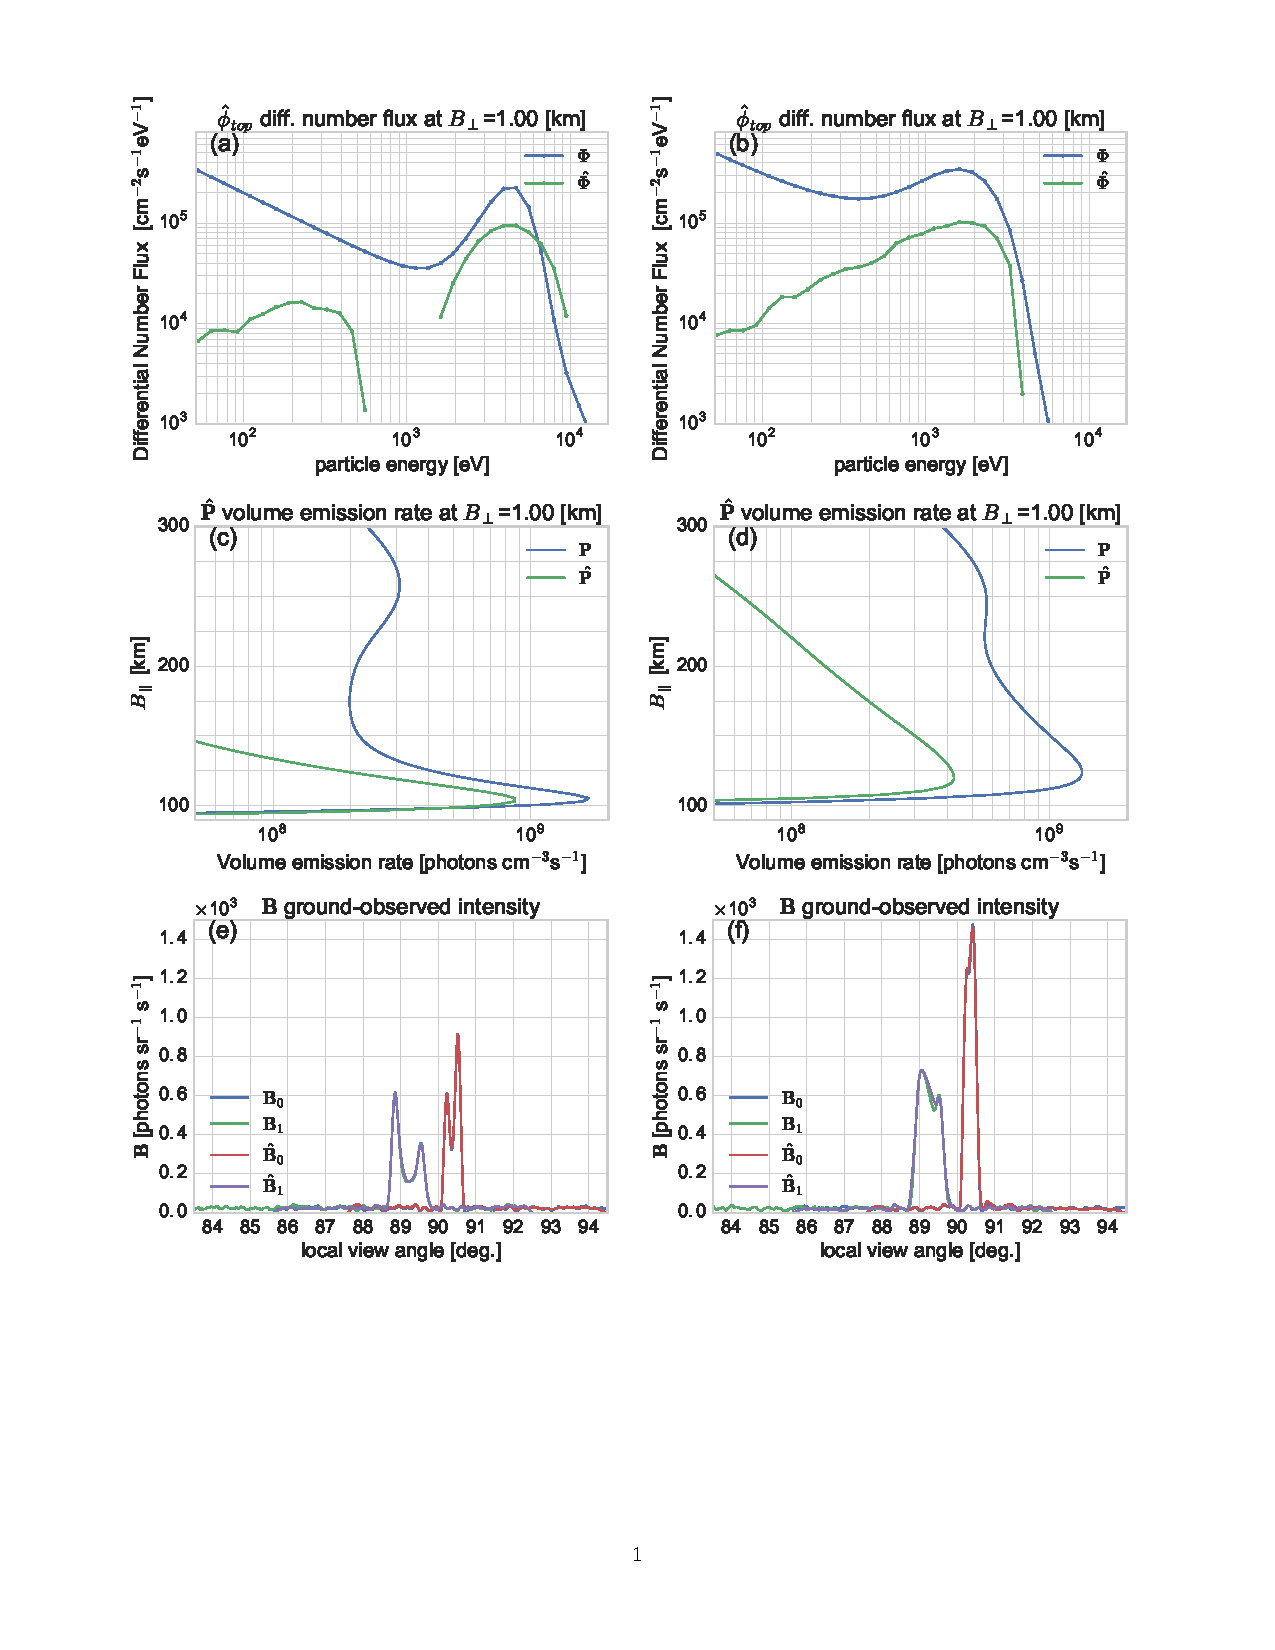
\includegraphics[trim=50 150 50 40,clip,height=0.875\textheight]{gfx/flamesim1d}
\caption{Flaming aurora simulation, 1-D cuts. 
(a)(b): Estimated differential number flux $\hat{\Phi}$.
(c)(d): Volume emission rate $\hat{\mathbf{P}}$. 
(e)(f): Ground-observed intensity $\mathbf{I}$ for characteristic energy $E_0\in\{4.5,1.6\}$~keV.}\label{fig:est1dflame}
\end{figure}

% python figure_trans2.py --load -m fwd optim eps
\subsection{Model and Inversion of Laterally Translating Aurora}\label{sec:transverse}
The laterally translating aurora simulation was configured with $E_0\equiv \unit[5]{keV}$  and $B_{\perp,0}\in$\{1.55, 3.75\}~km. 
%
\begin{figure}
\centering
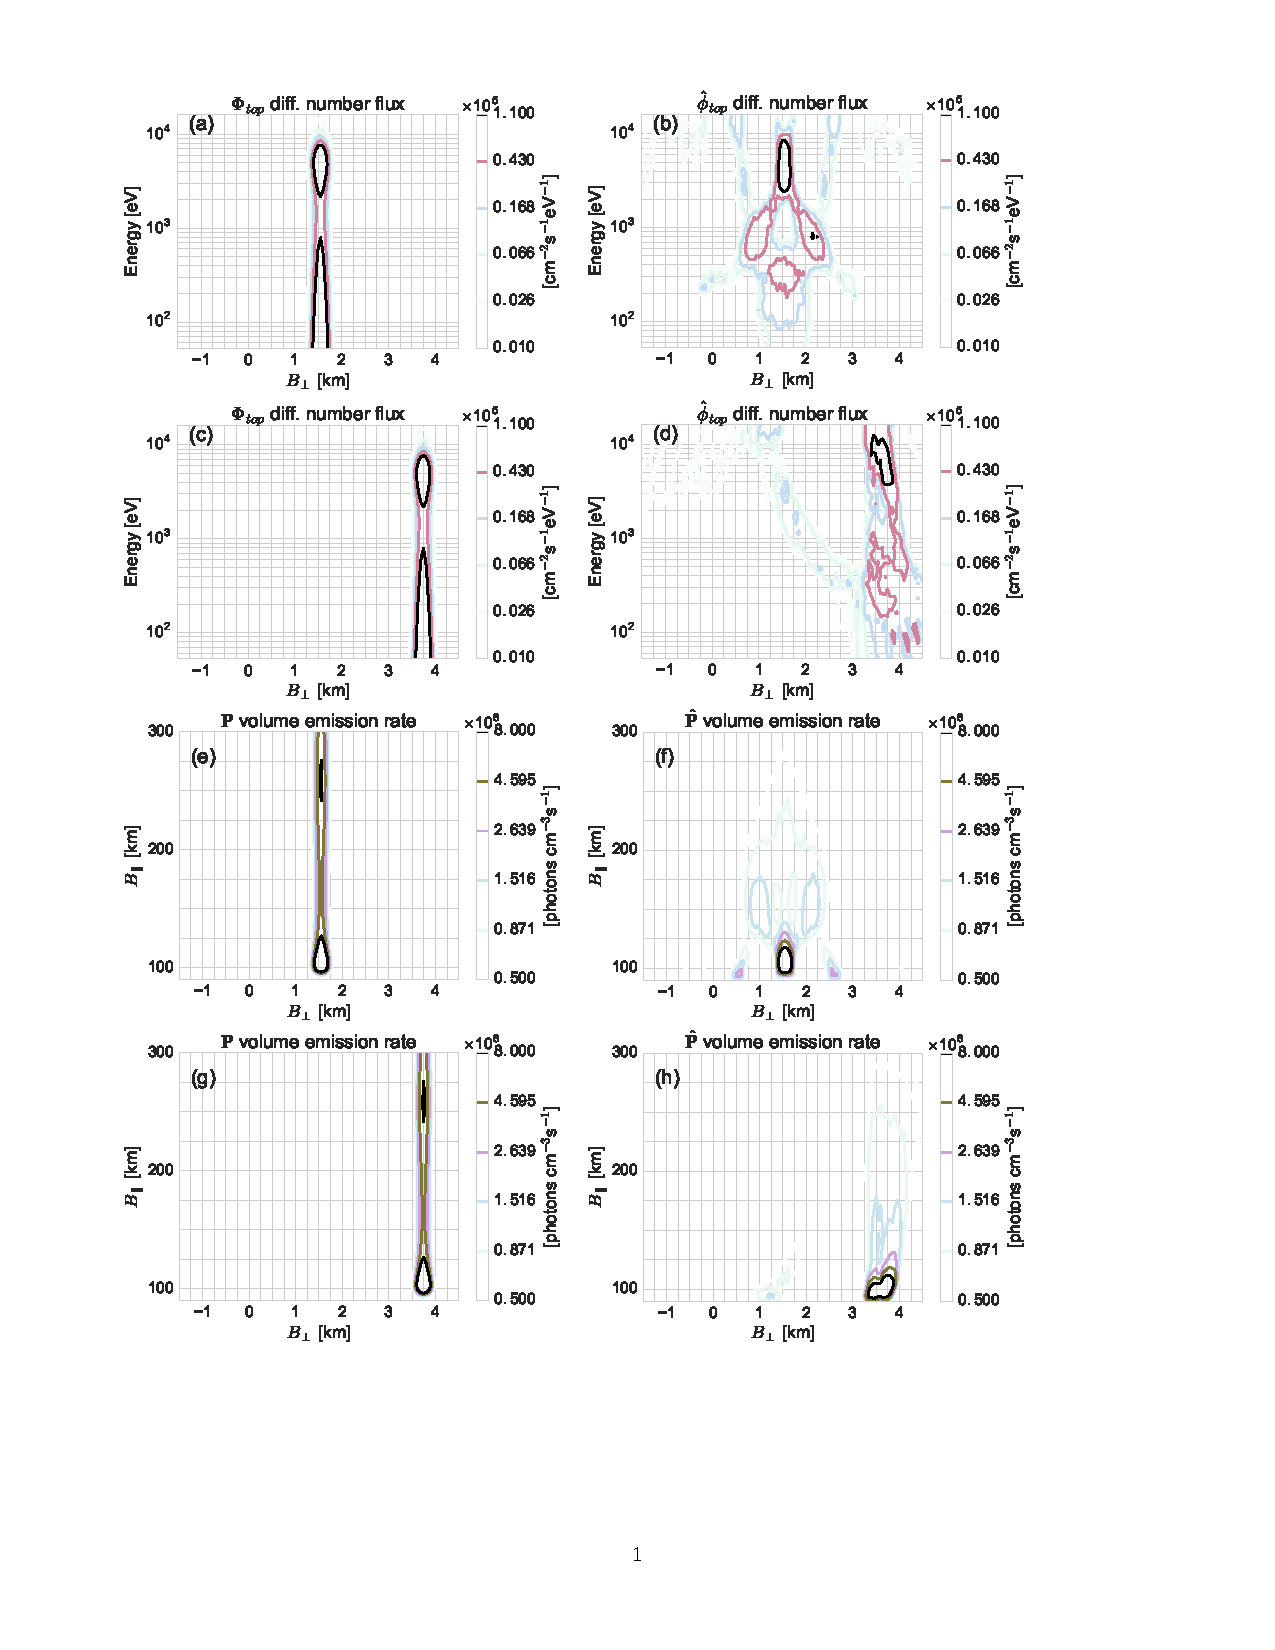
\includegraphics[trim=50 140 80 30,clip,height=0.875\textheight]{gfx/transversesim}
\caption{$B_\perp$ translating aurora simulation with characteristic energy $E_0 \equiv \unit[5]{keV}$ and $B_{\perp,0}\in$ \{1.55, 3.75\}~km. 
(a,c): differential number flux $\Phi_{top}$. (b,d): estimated differential number flux $\hat{\Phi}_{top}$. 
(e,g): forward modeled VER $\mathbf{P}$.  (f,h): estimated VER $\mathbf{\hat{P}}$.}%
\label{fig:JPB}
\end{figure}
%
Fig.~\ref{fig:JPB}(a)(c) show the input differential number flux $\Phi_{top}$, resulting in the volume emission rate $\mathbf{P}$ displayed in Fig.~\ref{fig:JPB}(e)(g). 
Fig.~\ref{fig:JPB}(b)(d) shows the estimated differential number flux $\hat{\Phi}_{top}$ using the L-BFGS-B algorithm and two cameras at $B_\perp \in\{0,3\}$ ~km.
Table~\ref{tab:Jestflame} describes the estimated differential number flux results.
The artifacts in $\hat{\Phi}_{top}$ and $\mathbf{\widehat{P}}$ come from the noise deliberately injected into the simulated $\mathbf{I}$. 
These artifacts are smaller in amplitude than the peak closest to the true answer, allowing for $\hat{\Phi}_{top,0}$ to be extracted despite the artifacts.
The estimated volume emission rate $\hat{\mathbf{P}}$ shown in Fig.~\ref{fig:JPB}(f)(h) has morphologically similar characteristics to the forward modeled volume emission rate in Fig.~\ref{fig:JPB}(e)(g), as expected. 


\section{Conclusions}\label{sec:concl}
This chapter shows results from a regularization scheme using the physics encapsulated in TRANSCAR modeled eigenprofiles in a two camera simulation, with testing extended to three cameras for future 3-D work.
We observed estimates of the peak differential number flux $\hat{\Phi}_{top,0}(B_{\perp,0},E_0)$ for an auroral arc in the common FOV of the cameras, with typical error less than 30\% for auroral arcs within $2.5^\circ$ from camera boresight on magnetic zenith. 
TRANSCAR is used in a linear basis expansion of log-spaced energy bins across an energy range observed in the most common auroral events, enabling future extension to incorporate incoherent scatter radar and other instruments to form a meta-instrument for observing the ionospheric short term and long term trends.
This basis expansion is used to regularize the poorly observed vertical dimension, simultaneously enabling  high spatial resolution in $B_\perp$, which is important for capturing the detail in dynamic dispersive auroral events with \unit[10]{ms} temporal scales.
The performance estimates of this feasibility study show that a two camera system at the Poker Flat Research Range with \unit[3]{km} camera separation can give new science insights on multiple fronts, including the highly dynamic electron beam structures driving into the ionosphere.
Specifically, we can estimate the characteristic energy and $B_\perp$ peak location of the differential number flux $\Phi_{top}$.
The new observation techniques include use of filtered broadband optical emissions to select only prompt emissions with fast, highly sensitive EMCCD cameras, enabling the use of high frame rates with cadence of order \unit[10]{ms}.
The modeled HiST instrument is shown to be capable of high resolution electron precipitation characteristic energy estimates along $B_\perp$ within suitable error bounds, while retaining the qualitative morphology of the differential number flux in the spatial and energy domains.
Future work includes extending this estimate to 3-D by utilizing 3-D phantoms in the forward model and 3-D inversion of the 2-D pixel intensity images from the cameras, along with a 3 camera phase II HiST deployment to Poker Flat Research Range for a multi-year autonomous deployment beginning in the 2017 auroral season.

